\documentclass[10pt,a4paper,twocolumn]{article}
\usepackage[margin=19mm,columnsep=6mm]{geometry}
\usepackage[T1]{fontenc}
\usepackage{lmodern}
\usepackage{ragged2e,sectsty}
\allsectionsfont{\raggedright}
\usepackage{microtype,amsmath,amssymb,graphicx,booktabs,longtable,array}
\usepackage[numbers,sort&compress]{natbib}
\usepackage[colorlinks=true,linkcolor=blue,citecolor=blue,urlcolor=blue]{hyperref}
\usepackage{caption,fancyhdr,float}
\usepackage{dblfloatfix}
\usepackage{listings}
\lstset{basicstyle=\ttfamily\footnotesize,breaklines=true,columns=fullflexible,
  keepspaces=true,showstringspaces=false,frame=single,aboveskip=5pt,belowskip=5pt}
\setcounter{dbltopnumber}{2}
\renewcommand{\dbltopfraction}{.9}
\renewcommand{\textfraction}{.05}
\renewcommand{\dblfloatpagefraction}{.8}
\graphicspath{{../figures/}}
\captionsetup{font=small,labelfont=bf,justification=raggedright,singlelinecheck=false}
\setlength{\parskip}{3pt}
\setlength{\parindent}{1em}
\setlength{\textfloatsep}{12pt}
\setlength{\floatsep}{9pt}
\pagestyle{fancy}
\fancyhf{}
\fancyhead[L]{\small Memory Under Interference}
\fancyhead[R]{\small Preprint -- Version 1.1}
\fancyfoot[C]{\thepage}
\setlength{\headheight}{14pt}
\newcommand{\MainRequests}{5,528}
\newcommand{\SmallCross}{3.12}
\newcommand{\SmallCrossCI}{[-3.12, 11.25]}
\newcommand{\SmallCrossN}{40}
\newcommand{\SmallCrossP}{1}
\newcommand{\SmallFullEnergy}{325.38}
\newcommand{\SmallOracleEnergy}{76.39}
\newcommand{\SmallEnergyReduction}{76.5}
\newcommand{\SmallEnergyDiff}{-249.00}
\newcommand{\SmallEnergyCI}{[-529.62, -127.49]}
\newcommand{\SmallPromptDiff}{-2.25}
\newcommand{\SmallPromptCI}{[-7.77, 2.86]}
\newcommand{\SmallPromptP}{0.44696}
\newcommand{\SmallInitialDiff}{-27.50}
\newcommand{\SmallInitialCI}{[-45.00, -10.00]}
\newcommand{\SmallInitialP}{0.033691}
\newcommand{\SmallTargetDiff}{-11.25}
\newcommand{\SmallTargetCI}{[-20.62, -2.50]}
\newcommand{\SmallTargetP}{0.056396}
\newcommand{\LargeCross}{8.97}
\newcommand{\LargeCrossCI}{[3.21, 16.67]}
\newcommand{\LargeCrossN}{39}
\newcommand{\LargeCrossP}{0.03125}
\newcommand{\LargeFullEnergy}{154.16}
\newcommand{\LargeOracleEnergy}{50.20}
\newcommand{\LargeEnergyReduction}{67.4}
\newcommand{\LargeEnergyDiff}{-103.96}
\newcommand{\LargeEnergyCI}{[-152.30, -77.58]}
\newcommand{\LargePromptDiff}{2.64}
\newcommand{\LargePromptCI}{[-1.22, 6.30]}
\newcommand{\LargePromptP}{0.44156}
\newcommand{\LargeInitialDiff}{-2.50}
\newcommand{\LargeInitialCI}{[-17.50, 12.50]}
\newcommand{\LargeInitialP}{1}
\newcommand{\LargeTargetDiff}{-2.50}
\newcommand{\LargeTargetCI}{[-10.00, 4.39]}
\newcommand{\LargeTargetP}{0.63525}
\newcommand{\EmbeddingMRR}{0.7364}
\newcommand{\LexicalMRR}{0.5163}

\title{\vspace{-1cm}Memory Under Interference:\\Context Utilization, Specification Confusion, and Inference Efficiency in Small Code Language Models}
\author{}
\date{}

\begin{document}
\RaggedRight
\raggedbottom
\maketitle
\begin{abstract}
\RaggedRight
Increasing a language model's context makes more information available, but also
adds computational work and potentially competing instructions. When does that
extra information help a model solve the intended task? I investigate this
question through seven studies containing \MainRequests{} experimental requests
to quantized Qwen2.5-Coder 0.5B and 1.5B models running on a CPU laptop.
The experiments vary task descriptions, competing requirements, interruptions,
retained context and the placement of a code-only preference. In addition to
testing the requested solution, I test whether an incorrect answer satisfies a
competing requirement. This posthoc comparison finds \LargeCross{} percentage
points more such failures under competing than irrelevant context on 1.5B
(95\% task-bootstrap interval \LargeCrossCI{}). The 0.5B comparison is
inconclusive, and conservative assumptions about incomplete generations weaken
the 1.5B result. Retaining context using known relevance labels yields observed
estimated net CPU-package energy-per-correct-solution reductions of
\SmallEnergyReduction\% and \LargeEnergyReduction\% for 0.5B and 1.5B relative
to full history. Accuracy preservation remains uncertain, and differences in
prompt length, position, instructions and generated output confound attribution
of these reductions to retention alone. The results motivate evaluating memory
management through the answers it produces and its total computational cost,
alongside the relevance of the information it supplies.
\end{abstract}

\section{Introduction}
A coding assistant often receives more than the task it must solve. Its context
may contain earlier requests, examples, preferences and descriptions of related
problems. Keeping that history can preserve useful information. It can also
leave an old requirement beside a new one, increasing both the amount of text
to process and the chance of producing a plausible answer to the wrong problem.
The central question is whether the model uses the information needed for the
current task, rather than simply whether that information fits in its context.

This question grew out of \emph{Prompt-Energy}, my earlier experiment on how
prompt design relates to code correctness, token use, latency and estimated
inference energy. Its \href{https://github.com/buildgit17626-ctrl/Prompt-Energy}{implementation and report}
showed me why response length and the cost of unsuccessful attempts belong in
an evaluation of prompting. The present study asks a broader question: what
happens when context accumulates, and useful instructions appear alongside
irrelevant or competing information? Prompt-Energy motivated this work, but its
earlier observations are a separate dataset and are not pooled with the
experiments reported here.

Existing research shows that context position matters, that conversation
history can interfere with a new task, and that preferences become difficult
to follow in long interactions \citep{lost,interference,prefeval}. Other work
finds benefits from combining tasks \citep{multitask}. More context is therefore
neither inherently useful nor inherently harmful. I examine when its content
matters for two small local code models, using executable tests to distinguish
the requested behavior from a competing behavior.

Three questions guide the experiments. \textbf{RQ1:} Does additional task
content change correctness compared with similarly long neutral text?
\textbf{RQ2:} When an answer is wrong, does it satisfy a competing requirement
present in context? \textbf{RQ3:} How do context-retention policies and preference
instructions relate to correctness and computational cost?

The contribution is a set of paired code-task comparisons with inspectable
prompts and outputs, a cross-specification diagnosis of failures, and an
evaluation of cost per correct solution that includes failed attempts. The
comparisons reveal a mixed picture: the larger model's error distribution
changes in the complete cases, reduced context has lower observed estimated
cost, and several accuracy and reminder comparisons remain uncertain. The
posthoc analysis and its sensitivity to incomplete generations are reported
alongside the positive findings.

These results lead naturally to selective context management. To explore that
practical direction, I developed \emph{MemoryGraph}, a local prototype for
storing, organizing and retrieving historical information before it enters a
prompt. It combines lexical and embedding retrieval with a small entity graph
and lets the user inspect and approve selected memories. Its separate synthetic
evaluation measures ranking; downstream correctness and energy benefits remain
untested. I describe the \href{https://github.com/buildgit17626-ctrl/MemoryGraph}{existing prototype}
after the context experiments, connecting the measurement questions to a system
that could be evaluated in subsequent work.

\section{Related Work}
\paragraph{Using context and resolving instructions.}
Lost in the Middle shows that the position of relevant material can change
performance in question answering and retrieval \citep{lost}. Gupta et al.
study interference when conversational history switches tasks
\citep{interference}. Son et al. examine following several instructions in one
call and find that combining tasks can improve some outcomes \citep{multitask}.
These studies motivate comparisons that vary content as well as length.
My interruption experiment uses constructed transcripts rather than actual
earlier model execution, and my task bundles use smaller code models and
different workloads. Instruction Hierarchy studies training models to respect
instruction priorities \citep{hierarchy}; here I evaluate fixed models without
training an instruction hierarchy or testing adversarial security robustness.

\paragraph{Preferences and memory systems.}
PrefEval examines explicit and implicit preference following across longer
conversations \citep{prefeval}. My code-only preference is a narrower case,
with a scoring limitation discussed in the results. LongMemEval separates
indexing, retrieval and reading \citep{longmem}; EvalMem diagnoses encoding,
retrieval and generation failures \citep{evalmem}. LongMemEval-V2 extends memory
evaluation to accumulated experience in agent environments \citep{longmemv2}.
This work builds on the distinction between supplying information and using it,
rather than claiming that distinction as new. The main experiments begin with
already assembled prompts, so they examine code generation from available
context rather than the quality of a memory store.

\paragraph{Code correctness and computational cost.}
HumanEval evaluates generated functions through execution \citep{humaneval}.
EvalPlus adds tests and demonstrates that limited test coverage can change
both measured correctness and model rankings \citep{evalplus}. I use its
expanded benchmark with the Qwen2.5-Coder family \citep{qwen}. Inference-energy
research links cost to output length, prompts and runtime choices
\citep{sustainable}; a directly related 2026 study examines prompting, code
accuracy and environmental cost across small and open models \citep{slmenergy}.
The present measurements concern CPU-package energy on one laptop, without
transferring carbon or hardware conclusions from those studies.

\paragraph{Retrieving useful history.}
GraphRAG uses graph indexes and community summaries for questions about a
corpus \citep{graphrag}; Mem0 evaluates a more integrated persistent-memory
system \citep{mem0}. MemoryGraph is a smaller companion prototype with local
memory editing, ranking and a basic entity graph. Its role here is to identify
a practical next evaluation, not to claim the architecture or demonstrated
benefits of these systems. The accompanying related-work table records the
overlap and distinctions in this focused literature review; it is not a
systematic search or a claim of priority.

\section{Evaluation Framework}
The experiments separate four ideas. \emph{Availability} means that the needed
specification is present in the prompt. \emph{Retrieval} is the preceding act of
selecting stored material, illustrated separately by MemoryGraph.
\emph{Utilization} is measured through what the generated function does on its
tests. \emph{Efficiency} concerns tokens, latency and estimated CPU-package
energy. These observable outcomes do not measure internal memory capacity or
cognitive states.

An incorrect solution can still be informative. Suppose the target requires a
strict comparison, while a background task includes equality. A solution using
the inclusive rule is wrong for the target but may be right for that background
task. I test each complete response against target suite $T$ and alternative
suite $A$, distinguishing target-only pass, alternative-only pass, both pass
and both fail. An \emph{alternative-consistent failure} is thus an incorrect
target solution that satisfies the competing computational requirement.
``Specification confusion'' names this observed pattern, not a diagnosis of
the model's internal reasoning. Finite tests, extraction errors and ordinary
algorithmic mistakes remain relevant to interpreting every cell.

\begin{figure*}[t]
\centering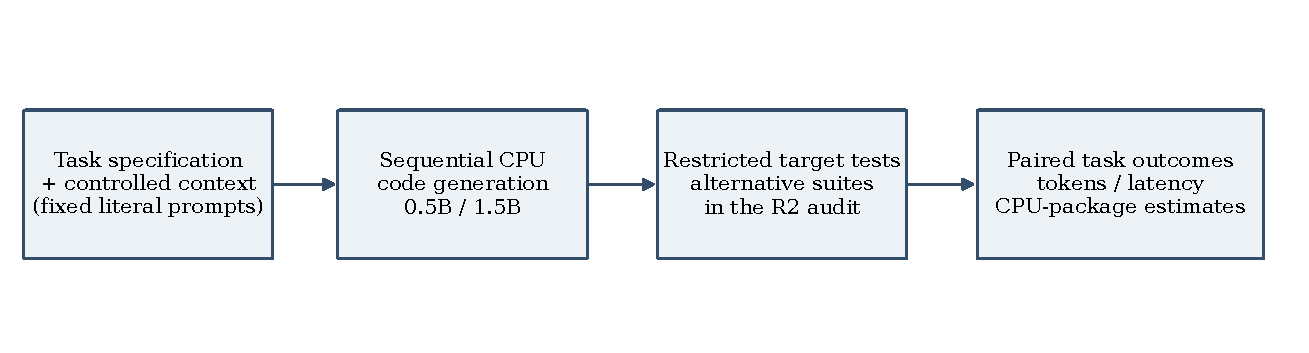
\includegraphics[width=\linewidth]{framework.pdf}
\caption{Observed-data framework. Target and context text are frozen before
generation. Scoring is separate and restricted. The additional alternative-suite
analysis uses saved outputs; it does not generate new answers.}
\label{fig:framework}
\end{figure*}

For each model and paired task $t$, let $y_{tc}$ denote a binary test outcome,
or the mean over the registered repeated cells in condition $c$. I report
$\widehat\Delta=|S|^{-1}\sum_{t\in S}(y_{ta}-y_{tb})$, preserving both arms
and all included cells within each resampled task. For energy, I ask how much computation was spent to obtain each correct
solution. The numerator includes the energy of failed attempts: discarding
those attempts would make an unreliable method look artificially cheap. For
the attempts with both energy and correctness readings, this cost is
\begin{equation}
\widehat C_c=\frac{\sum_{i\in I_c}E_i}{\sum_{i\in I_c}\mathbf{1}\{\text{correct}_i\}},
\end{equation}
where $I_c$ contains attempts with both energy and correctness readings. I report measurement coverage with the ratio and use successes from the same
covered attempts, so missing energy cannot silently change its denominator.

\section{Experimental Methodology}
\subsection{Models, tasks and execution}
The models are \texttt{qwen2.5-coder:0.5b} and
\texttt{qwen2.5-coder:1.5b}, both Q4\_K\_M quantizations, with exact model
digests recorded in frozen jobs. Inference used Ollama on Windows 11, an Intel
i5-13420H CPU and approximately 16 GB RAM, with eight inference threads and
\texttt{num\_gpu=0}. Generation was sequential, with randomized interleaved
condition schedules. Recorded block-start checks observed AC power and Best
performance; these snapshots do not prove an invariant host state throughout
every request. Decoding settings, templates, native token counts, raw outputs
and retry records are retained.

An experimental request means one scheduled task/condition/model/sample call;
a retry does not create another independent observation. The seven studies
contain the following requests, including documented failures: isolated strategy comparison, 1,968; initial
context load plus its isolation controls, 280; task bundles, 1,040; retention,
400; revised semantic interference plus isolation, 1,040; static interruptions
plus isolation, 400; and preference placement, 400. These sum directly to
\MainRequests{}. Pilots are separate observations. The revised cache study
saved 76 of 400 planned full requests and is a partial appendix diagnostic.
The detailed inventory and unfinished studies are documented in the appendix.

The isolated strategy study covers all 164 HumanEval+ tasks, comparing P1 and
P3\_1 with three temperature-0.2 samples per task/model, context 8,192 and output
budget 2,048. The strategies differ in both instructions and an external
example, so this is not a pure example-effect contrast. Initial context load
uses 20 held-out-eligible tasks per model, with fresh temperature-0
no-filler outcomes; the sample used for selection is never the isolation
comparator. Its model-selected populations and weaker renamed-specification
distractors remain separate from the revised designs.

In my later studies, I use the original fixed 40-task roster for both models. I
use temperature 0 and one generation per task-condition-model. Context is
32,768 for task bundles, 16,384 for retention/revised interference/interruptions,
and 8,192 for preferences. Output budgets are 2,048 except that active bundles
receive 2,048 per requested function. Explicit context reservations and native
prompt counts detect mismatches; invalid calls are reported, not repaired by
silent parameter changes.

\subsection{What the context comparisons test}
To separate reading extra tasks from solving them, passive load adds other task
descriptions, while active load requests their
functions as well. $K\in\{2,3,4,6\}$; neutral filler matches passive input
length. Target placement and companions are fixed. Active requests do more
output work, so focal-target, per-function and whole-bundle endpoints are kept
distinct. Reused component-isolation outputs are lookup references, not newly
measured bundle execution.

To test whether a competing requirement changes the answer, the revised
interference experiment crosses three filler types, filler-token targets
1,000/2,000 and target beginning/end, with matched isolation controls. Competing
descriptions change a computational requirement, such as strict versus
non-strict comparison or inclusive versus exclusive boundaries. Alternative
references and distinguishing inputs were validated. The model sees descriptions,
not the alternative implementation or hidden tests. Related/irrelevant labels
are authored coarse categories; they are not calibrated semantic similarity.
Filler budgets do not guarantee identical complete input lengths across every
wrapper, an important limit on attributing differences solely to content.

To examine the cost of keeping history, I compare full history, target/query
only, verbatim target replay,
lossless target-format compaction, and oracle retention. Oracle retention means
selecting context using known relevance labels: the target specification and
preference are kept without having to discover which history is relevant. Eight fixed distractor
descriptions form full history. No-history omits the explicit code-only
preference, while the oracle retains target, preference and final query.
Compaction removes redundant target formatting and drops other history; it is
not semantic summarization of a conversation. These policies jointly change
length, position, repetition and sometimes instruction content.

To examine returning to a task after intervening descriptions, the static
interruption conditions contain neutral material, one similar competing
description, one other-domain description, or three other-domain descriptions.
Loaded complete input counts match, with the same target and final instruction.
Descriptions and acknowledgements are literal transcripts, not tasks executed
earlier by the model. Similarity, count and diversity are not fully crossed.
Finally, to test whether a reminder helps with an output preference, preference
placement compares absent, immediate, buried, replayed and corrected
code-only instructions while preserving the target/query and distractor history.

\subsection{Statistics, exclusions and energy}
Intervals use 2,000 paired task-bootstrap draws with seed 1732. Binary pairs use
exact discordant-pair McNemar tests; task means over repeated cells use exact
paired sign swaps. Holm correction is within specified families: two isolated
strategy tests, two initial-load primary tests, two revised-interference primary
tests, six retention tests and six interruption tests. The new cross-pass audit
uses four posthoc tests. These corrections do not control every analysis ever
examined in the project. Intervals are pointwise, not simultaneous family
intervals. Null tests do not establish equivalent accuracy.

I preserve failed requests and capped generations. Caps are nonpasses
for bounded correctness endpoints but unknown for the uncensored cross-pass
taxonomy. API, input or evaluator-infrastructure failures are missing for
valid-input accuracy and separately reduce operational yield. I report cap
exclusion, optimistic bounded-correctness scenarios, adverse cross-pass coding,
independently labelled eligibility subsets, and exclusion of the documented
HumanEval/32 oracle anomaly. The expanded-test adapter and sandbox restrictions
remain part of the operational outcome, not an infallible correctness oracle.

HWiNFO CPU Package Power was logged at a nominal 500 ms interval. Gross energy
uses trapezoidal integration; net estimates subtract the block-start idle
baseline over the request window. Approximate post-load and total windows are
both retained. End/midpoint subtraction, drift exclusions and short-window
exclusions are secondary sensitivities. Per-condition totals are preferred to
precise interpretations of short individual windows. The registered primary
cache-energy experiment is incomplete; retention energy remains descriptive or
posthoc. No whole-system electricity, carbon, GPU or cloud inference is measured.

\section{Contextual Interference}
\subsection{Does task content matter beyond length?}
The task-bundle experiment asks whether similarly long contexts behave
differently when the extra text describes other problems. Figure~\ref{fig:m1}
compares correctness of the designated target function under passive, active and
neutral conditions. Passive-minus-filler estimates tend to be negative across
$K$ in this roster, but many adjusted comparisons are inconclusive. The 0.5B
$K=6$ estimate is $-25$ percentage points, conditional interval $[-37.5,-12.5]$,
with Holm $p=0.015625$ in its eight-comparison posthoc family. This is evidence about the fixed task combinations tested here, rather than
a general penalty for multitasking.

Tasks recur in several bundles, and all bundles are connected through shared
members. The bootstrap therefore describes variation across target tasks while
keeping their companions fixed; it cannot supply uncertainty for independently
resampled bundles. Changing $K$ also changes
which companion functions appear. Active per-function fractions and whole-bundle
successes are reported against the same components' isolation outcomes in the
archive, rather than equating a passive focal pass with a complete active bundle.
The additional output budget and repeated component references limit cost
comparisons. The shared companions and additional output work are important alternative
explanations when comparing bundle performance and cost.

\begin{figure*}[t]
\centering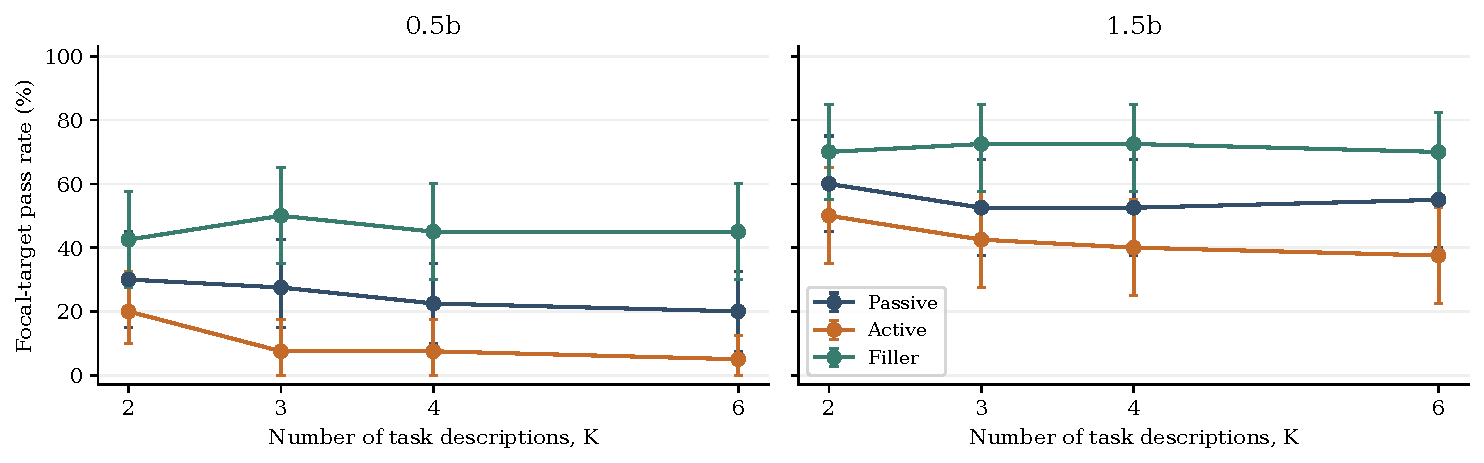
\includegraphics[width=.95\linewidth]{m1.pdf}
\caption{M1 focal-target pass rates, 40 anchors per model/mode/$K$. Whiskers are
conditional task-bootstrap intervals with overlapping fixed companions. Active
mode requests $K$ functions and has a larger output budget. These are not
dependence-robust independent-bundle confidence intervals.}
\label{fig:m1}
\end{figure*}

\subsection{Does a wrong answer follow the competing requirement?}
The first comparison asks whether competing descriptions reduce target
correctness relative to irrelevant descriptions. The registered difference is
\SmallTargetDiff{} percentage points for 0.5B, interval \SmallTargetCI{}, Holm
$p=\SmallTargetP{}$, and \LargeTargetDiff{} for 1.5B, interval
\LargeTargetCI{}, Holm $p=\LargeTargetP{}$. Both comparisons have 40 paired
tasks averaged over four length/position cells. A pointwise interval excluding
zero can coexist with an adjusted test that does not reject; both are reported.
Figure~\ref{fig:matrix} shows the cell-level outcomes without treating them as
independent task replications.

\begin{figure*}[t]
\centering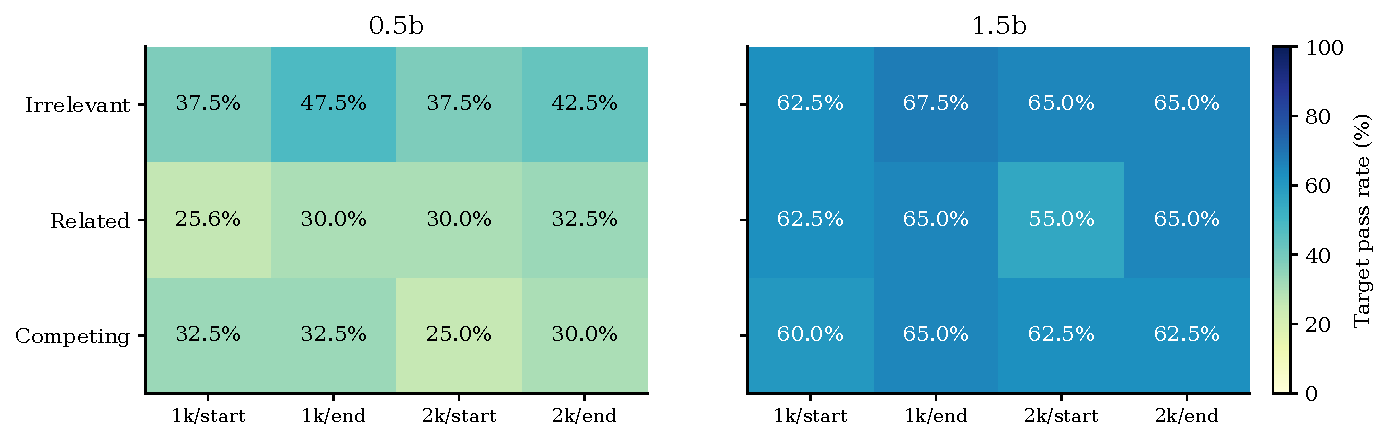
\includegraphics[width=.98\linewidth]{interference_matrix.pdf}
\caption{Revised M3/R2 target pass rates. Columns are filler-token targets and
target positions, not total input length. Cells contain 40 scheduled tasks;
one related-context API failure leaves 39 valid outcomes in its cell. Caps are
bounded-endpoint nonpasses. Per-cell denominators and intervals accompany the
figure's CSV source table.}
\label{fig:matrix}
\end{figure*}

Overall accuracy does not describe which requirement a wrong answer follows.
Testing the same saved programs against the competing specification reveals a
different pattern. For 1.5B, the posthoc difference in
distractor-only success between competing and irrelevant contexts is
\LargeCross{} percentage points, interval \LargeCrossCI{}, across
\LargeCrossN{} complete matched tasks; Holm $p=\LargeCrossP{}$. Versus
isolation, the estimate is 9.62 points, interval $[3.21,17.95]$, in the same
four-test family. The 0.5B competing-minus-irrelevant estimate is
\SmallCross{} points, interval \SmallCrossCI{}, $p=\SmallCrossP{}$.
The stronger 1.5B error-type association therefore does not imply a similarly
large change in its overall target pass rate.

Figure~\ref{fig:cross} includes every scheduled response, whereas complete-case
inference requires all paired cells. No response passes both suites in this
dataset. Figure~\ref{fig:worked} makes one alternative-only outcome concrete.
The target specification is present and marked as the only function to implement,
yet the saved body uses the competing inclusive boundary. A second audited
1.5B response reverses parenthesis-group order as required by its alternative.
These selected examples illustrate the test categories; they do not estimate
their prevalence or reveal why the model produced those programs.

\begin{figure*}[t]
\begin{minipage}[t]{.48\linewidth}
\RaggedRight
\small\textbf{Actual pair: HumanEval/0.}
The target requirement reads: ``Check if in given list of numbers, are any two
numbers closer to each other than given threshold.'' Its reference uses a
strict inequality. The background alternative reads: ``Return whether two
distinct list positions have absolute difference less than OR EQUAL TO threshold.
Equality is included.''

\textbf{Validated distinguishing input:}
\texttt{numbers=[1.0, 2.0], threshold=1.0}.
The target expects \texttt{False}; the alternative expects \texttt{True}.
The archived generated program fails the target suite and passes the alternative
suite; separate saved witness checks reproduce that classification.

\textbf{Source:} 0.5B, competing 1k/start condition; saved call key begins
\texttt{34303c8e4927}. Full key, prompt, original code, test outcomes and hashes
are in \texttt{examples/provenance.json}. No new execution was used for this figure.
\end{minipage}\hfill
\begin{minipage}[t]{.49\linewidth}
\RaggedRight
\vspace{0pt}
\lstinputlisting[language=Python,basicstyle=\ttfamily\scriptsize]{../examples/generated-code-excerpt.txt}
\small The executable text is unchanged; only the function docstring is omitted
from this listing. The complete saved response retains the original target
docstring, making the mismatch between stated requirement and body inspectable.
\end{minipage}
\caption{Worked cross-specification diagnosis from existing audited evidence.
The model saw the alternative description, not its implementation or hidden
tests. The construction repeats that description to reach its filler budget;
this repetition is part of the tested context (Appendix~\ref{app:prompts}).}
\label{fig:worked}
\end{figure*}

\begin{figure*}[t]
\centering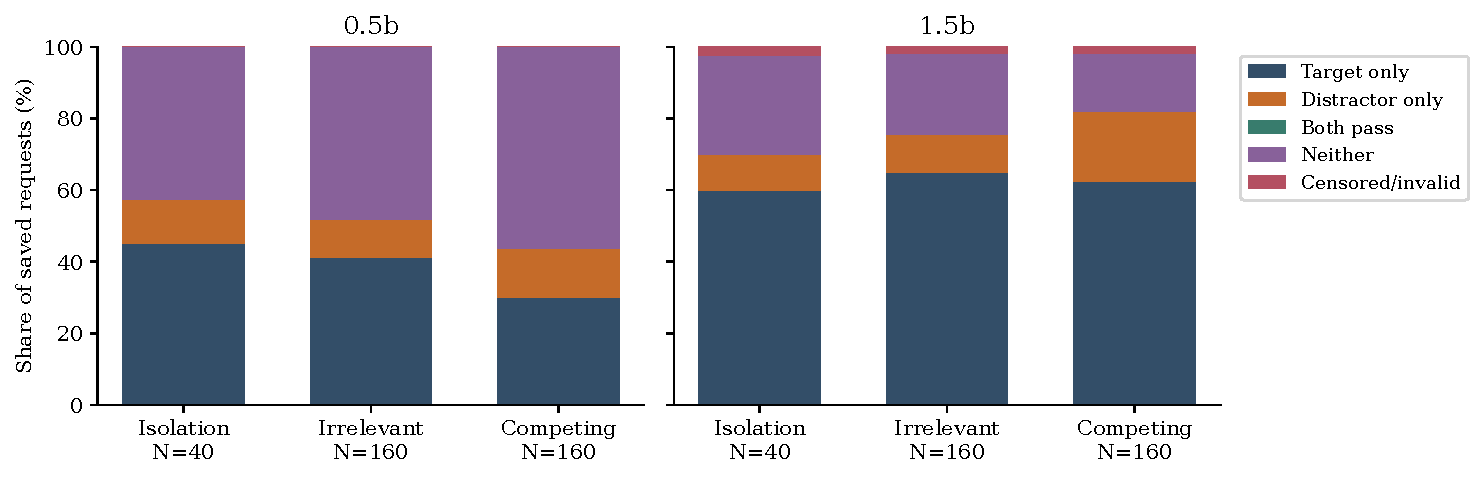
\includegraphics[width=.98\linewidth]{cross_outcomes.pdf}
\caption{Descriptive cross-specification cells. Isolation has 40 requests per
model; loaded groups have 160. Censored/invalid outcomes remain visible and
both-pass counts are explicitly zero. These stacked shares are not independent
request-level inferential estimates; paired effects use task means.}
\label{fig:cross}
\end{figure*}

Incomplete or invalid responses leave some classifications unknown. As a
conservative check, I assign those unknown outcomes in whichever way weakens
the observed association: none counts as an alternative-only success under
competing context, and every unknown control does. This yields a 1.5B
difference of 6.88 points over all 40 tasks, scenario interval
$[-0.02,15.00]$, adjusted $p=0.53125$. The favorable assignment gives 10.62
points, interval $[3.75,18.75]$. These adverse and favorable assignments describe sensitivity to missing
outcomes. They are hypothetical classifications, not repaired responses or a
formal confidence set for missingness.
The complete-case result is therefore suggestive but not robust to all cap
assignments (Figure~\ref{fig:paired}).

\begin{figure*}[t]
\centering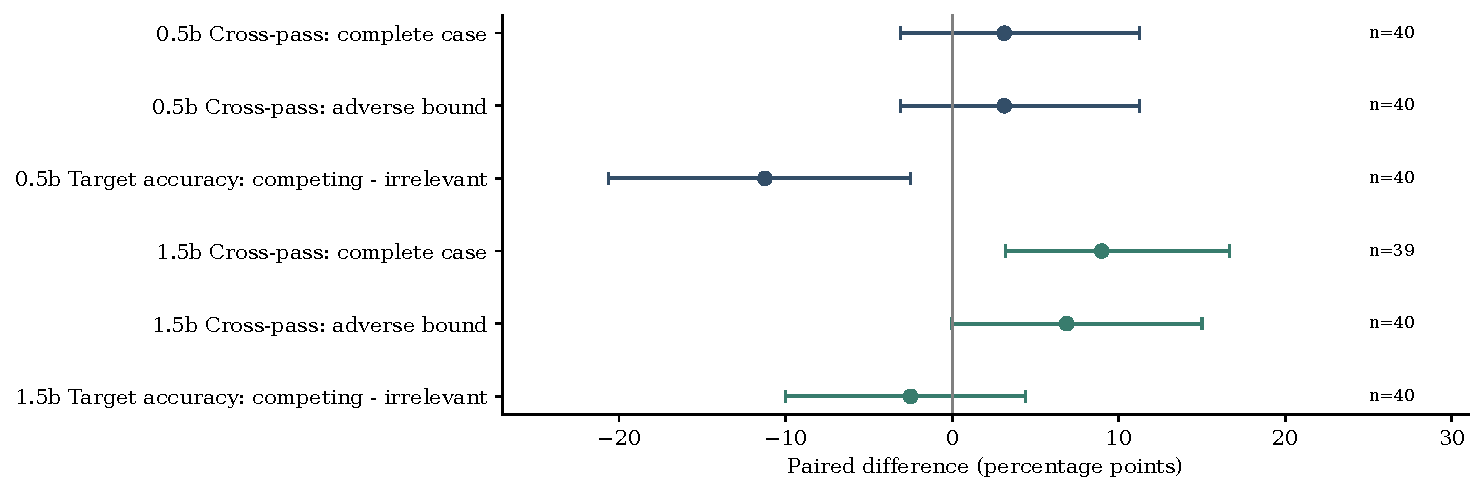
\includegraphics[width=.98\linewidth]{paired_effects.pdf}
\caption{Paired task effects for revised interference, with 95\% pointwise
bootstrap intervals. Cross-pass comparisons are posthoc. Adverse-bound rows
assign censored indicators against the observed association; target accuracy
uses registered bounded outcomes. Different endpoints and populations are
labelled rather than pooled.}
\label{fig:paired}
\end{figure*}

\subsection{Initial context load and static interruptions}
Initial context load shows a near-minus-irrelevant estimate of
\SmallInitialDiff{} points for 0.5B, interval \SmallInitialCI{}, Holm
$p=\SmallInitialP{}$, and \LargeInitialDiff{} for 1.5B, interval
\LargeInitialCI{}, $p=\LargeInitialP{}$. These selected populations and weaker
distractors cannot be pooled with the revised semantic experiment. Differences in selection and distractor construction prevent interpreting the
larger initial estimate as a stronger version of the revised experiment.

The six primary interruption comparisons do not establish a corrected effect.
For example, three other-domain descriptions versus neutral material on 1.5B
give $-15$ points with interval $[-27.5,-2.5]$, but Holm $p=0.421875$.
This illustrates the distinction between pointwise intervals and family tests.
Its constructed history and coarse domain labels also preclude a general claim
about real task switching. Isolated strategy differences are similarly
uncertain: P3\_1 minus P1 is \SmallPromptDiff{} points on 0.5B, interval
\SmallPromptCI{}, and \LargePromptDiff{} on 1.5B, interval
\LargePromptCI{}. Together, these comparisons show why neither additional history nor a reminder
can be assumed to have a consistent effect across the tested settings.

\section{What Is Gained by Keeping Less Context?}
The retention experiment compares ways of presenting the same target amid a
fixed history. It asks whether keeping less information, or replaying the target,
changes correctness and the cost of obtaining a correct answer. All five policies are shown in Table~\ref{tab:r1} and Figure~\ref{fig:r1}.
Oracle retention's correctness difference from full history is $+7.5$ points
on 0.5B, interval $[-5,22.5]$, and $+2.5$ on 1.5B, interval $[-10,15]$.
All six registered replay/oracle/compaction accuracy contrasts have Holm
$p=1$. Replay is not established to improve accuracy, and neither is
equivalent accuracy established by these wide intervals.

\begin{table*}[t]
\centering\small\begin{tabular}{llrrrr}
\toprule
Model & Policy & Correct/40 & Input & Output & Net mWh/correct \\
\midrule
0.5B & Full history & 14/40 & 1327.8 & 448.4 & 325.38 \\
0.5B & Target/query & 19/40 & 170.6 & 501.2 & 157.52 \\
0.5B & Verbatim replay & 15/40 & 1467.8 & 225.2 & 226.92 \\
0.5B & Lossless compaction & 16/40 & 177.0 & 193.7 & 79.29 \\
0.5B & Oracle retention & 17/40 & 183.6 & 196.0 & 76.39 \\
\midrule
1.5B & Full history & 22/40 & 1327.8 & 69.1 & 154.16 \\
1.5B & Target/query & 28/40 & 170.6 & 301.6 & 161.21 \\
1.5B & Verbatim replay & 23/40 & 1467.8 & 75.2 & 163.53 \\
1.5B & Lossless compaction & 22/40 & 177.0 & 64.6 & 53.00 \\
1.5B & Oracle retention & 23/40 & 183.6 & 63.6 & 50.20 \\
\midrule
\bottomrule
\end{tabular}

\caption{R1 observed outcomes, 40 tasks per policy/model. Tokens are means.
Energy is HWiNFO estimated net CPU-package mWh per correct solution, including
failed-attempt energy. All 40 requests have readings in each row. Confidence
intervals and paired contrasts are reported separately.}
\label{tab:r1}
\end{table*}

Although the accuracy comparisons remain uncertain, the observed cost ratios
differ substantially.
Estimated net energy per correct solution is \SmallFullEnergy{} mWh for full
history and \SmallOracleEnergy{} for oracle retention on 0.5B; corresponding
1.5B values are \LargeFullEnergy{} and \LargeOracleEnergy{} mWh. These ratios
correspond to observed estimated-cost reductions of \SmallEnergyReduction\%
and \LargeEnergyReduction\%, computed as $100(1-C_{\rm oracle}/C_{\rm full})$.
They are descriptive reductions, without an established accuracy-preservation
guarantee. Paired
oracle-minus-full ratio differences are \SmallEnergyDiff{} mWh, interval
\SmallEnergyCI{}, and \LargeEnergyDiff{} mWh, interval \LargeEnergyCI{}.
These intervals resample complete paired task clusters and recompute both
ratios; they are not intervals on the energy of successful requests alone.

\begin{figure*}[t]
\centering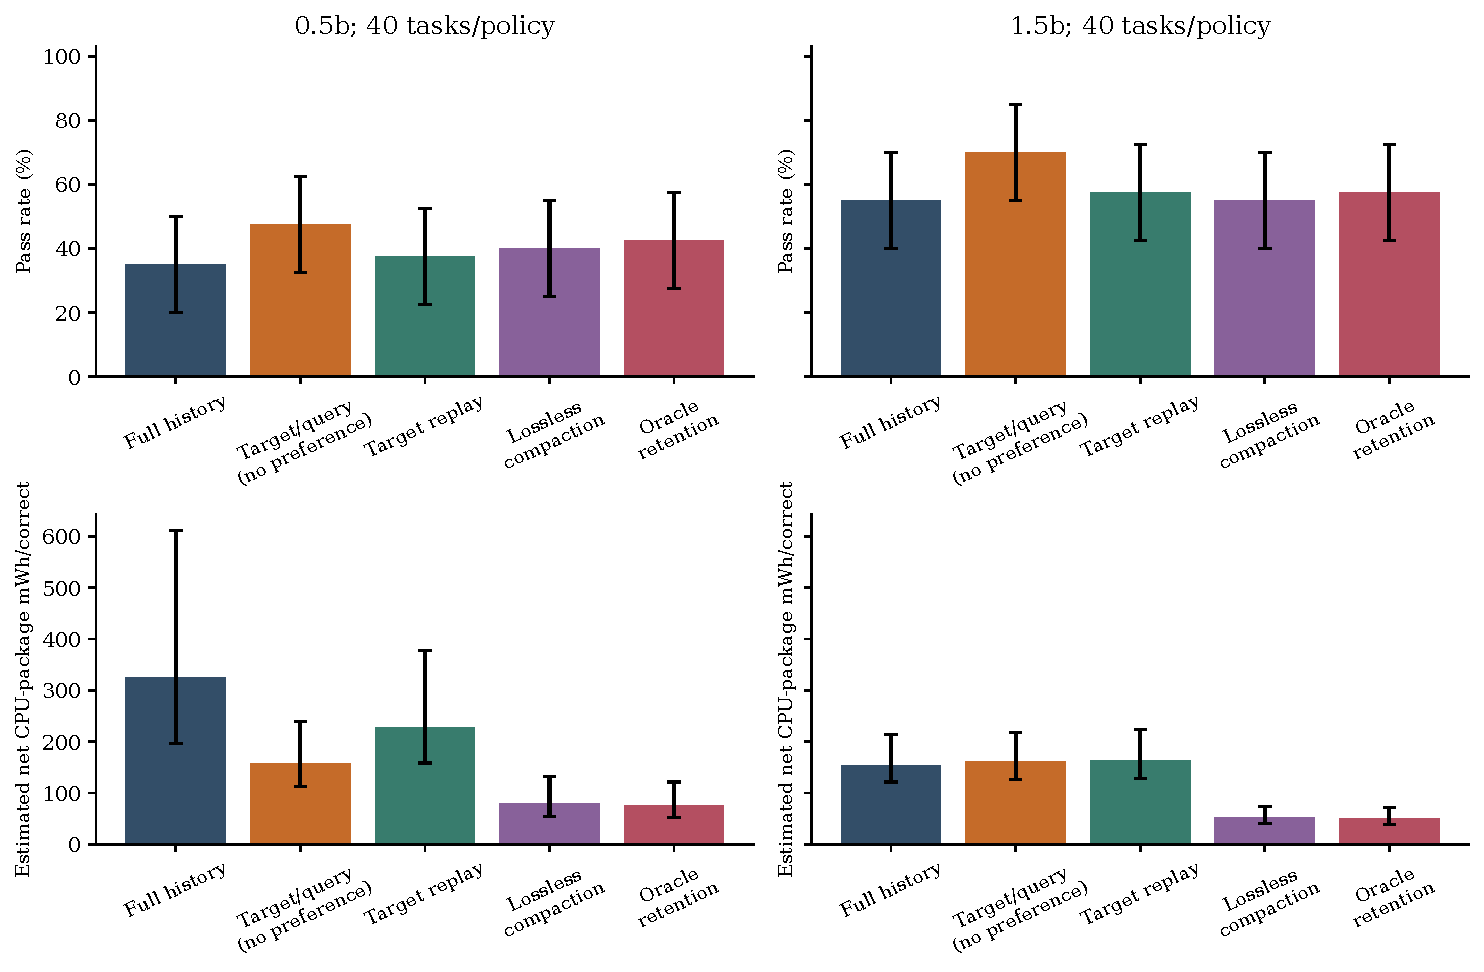
\includegraphics[width=.93\linewidth]{r1_policies.pdf}
\caption{R1 correctness and estimated net CPU-package energy per correct
solution, with pointwise task-bootstrap intervals. A shorter retained prompt
does not isolate memory-policy quality: instructions, input position and output
length also differ. Ratios include every covered attempt's energy. Model panels
use common scales within each row; target/query omits the code-only preference.}
\label{fig:r1}
\end{figure*}

End- and midpoint-baseline subtraction retain the lower oracle cost estimates
in these data. Excluding drifted observations also retains the direction, on
smaller matched populations. Cap exclusion reduces the 0.5B paired difference
to approximately $-112.65$ mWh over 35 tasks. Some short-window-excluded 0.5B
ratio draws have zero correct solutions; finite intervals are deliberately
left unavailable. In 1.5B oracle retention, removing short windows leaves only
18 of 40 calls. It preferentially removes cheap requests, rather than producing
a cleaner estimate for the original population.

These cost differences make selective context management worth investigating,
but the oracle has an advantage a practical system must earn: it is told what
matters. Full history and the reduced policies differ in input
length and recency. No-history omits the code-only instruction and produces
more output tokens; compaction only changes formatting of retained target text.
Generation budgets, output caps and runtime overhead can also influence ratios.
No automated retrieval/indexing cost is included. The sample Pareto display
(Figure~\ref{fig:pareto}) summarizes observed policy trade-offs, not a
population-optimal frontier or proof of accuracy-preserving energy savings.

\begin{figure*}[t]
\centering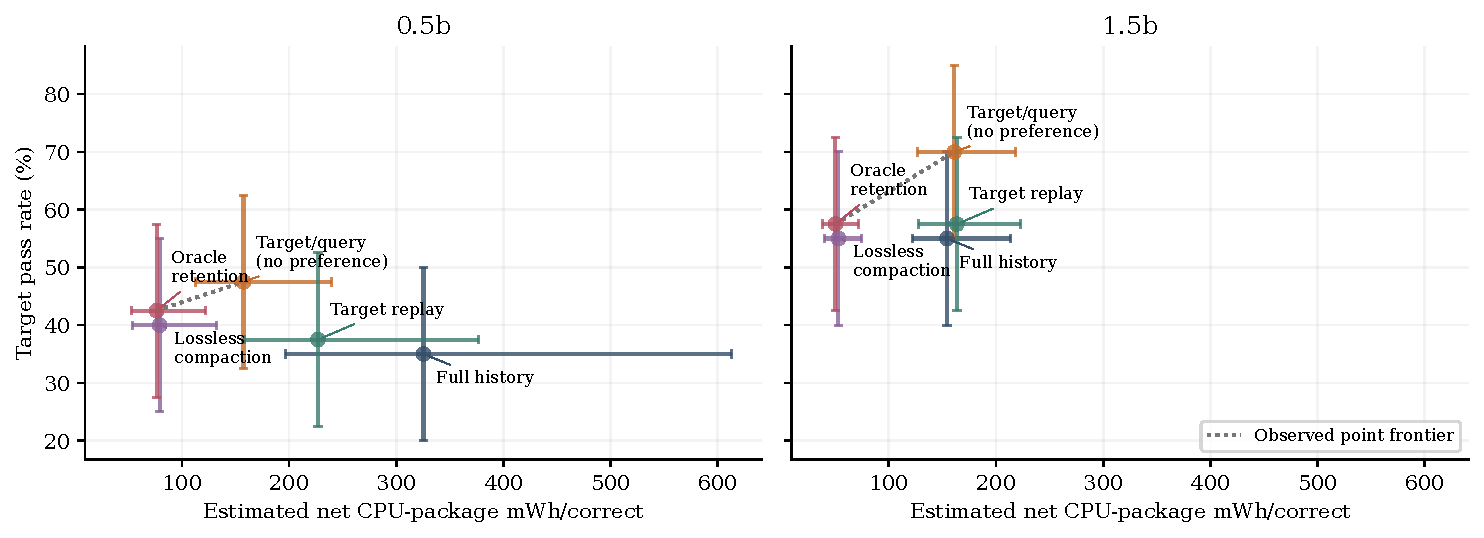
\includegraphics[width=.98\linewidth]{pareto.pdf}
\caption{Descriptive R1 accuracy--energy plots, separately by model, 40 tasks
per policy. Energy is HWiNFO estimated net CPU-package mWh/correct. Horizontal
and vertical whiskers are marginal bootstrap intervals, not joint confidence
regions. Both model panels share the same axes. The dotted frontier uses
sample point estimates only.}
\label{fig:pareto}
\end{figure*}

\section{What Does the Preference Test Measure?}
I designed the preference experiment to ask whether a buried code-only
instruction is followed less often than an immediate instruction, and whether
repeating it helps. The registered score accepts parseable Python defining the
target function only when it is not enclosed in Markdown fences. It accepts
zero out of 400 full-study responses: every output fails this particular rule,
leaving no variation for either primary placement/reminder comparison. The instruction
asks for code only but does not explicitly prohibit Markdown fences. The zero score therefore cannot be read as evidence that every preference
was forgotten.

To understand the zero scores, I retained the original metric and added a
separate posthoc format check recording fences,
outside prose, comments, docstrings and a fence-tolerant syntax predicate.
For 1.5B, each explicit-preference condition has 40/40 fence-tolerant outputs,
whereas no-preference has 21/40. For 0.5B, explicit conditions range from
36/40 to 39/40, versus 15/40 without the preference. These descriptive
differences do not establish long-term retention: immediate, buried and replayed
conditions also differ in rendered wording and position, and the registered
strict contrasts remain unchanged. Buried/replay comparisons under the
fence-tolerant predicate do not establish a benefit after correction.

Comments and docstrings can be legitimate code or explanatory content.
Mechanical counts do not replace human semantic adherence annotations. Joint
correctness-and-adherence outcomes are provided under each definition rather
than silently selecting the most favorable score. A zero-width empirical
bootstrap interval at an all-zero/all-one sample is not certainty about a
population rate. This scoring-definition problem is itself an honest limitation
of the experiment.

\section{MemoryGraph: A Practical Direction for Context Selection}
\subsection{From Oracle Retention to Practical Memory Retrieval}
MemoryGraph addresses the step before generation: choosing useful historical
information without automatically passing the entire history to the model. Its
\href{https://github.com/buildgit17626-ctrl/MemoryGraph}{implementation} is
examined at commit
\texttt{c569143ec6be1c767a2c56c59c936f85bd1fc1cb}. It stores editable local
plain-text memories; TF-IDF and pretrained sentence embeddings rank candidates.
A NetworkX bipartite graph links memories to a small fixed entity vocabulary.
The graph-assisted method adds a bounded bonus to lexical scores for shared
entities. This is not full GraphRAG, automatic memory extraction, or learned
feedback adaptation. Logistic regression and random-forest pipelines are
evaluation baselines, not a demonstrated learned online memory controller.

User control matters because a highly ranked memory may still be obsolete,
conflicting or unwanted in the current context. The interface exposes selected
text and requires explicit approval before a
local Ollama response comparison. Limited warnings detect explicit pytest versus
unittest and VS Code versus PyCharm preference conflicts; they do not resolve
arbitrary contradictions. No usability, trust, personalization or energy benefit
was measured. Figure~\ref{fig:mg} describes the existing components only.

\begin{figure*}[t]
\centering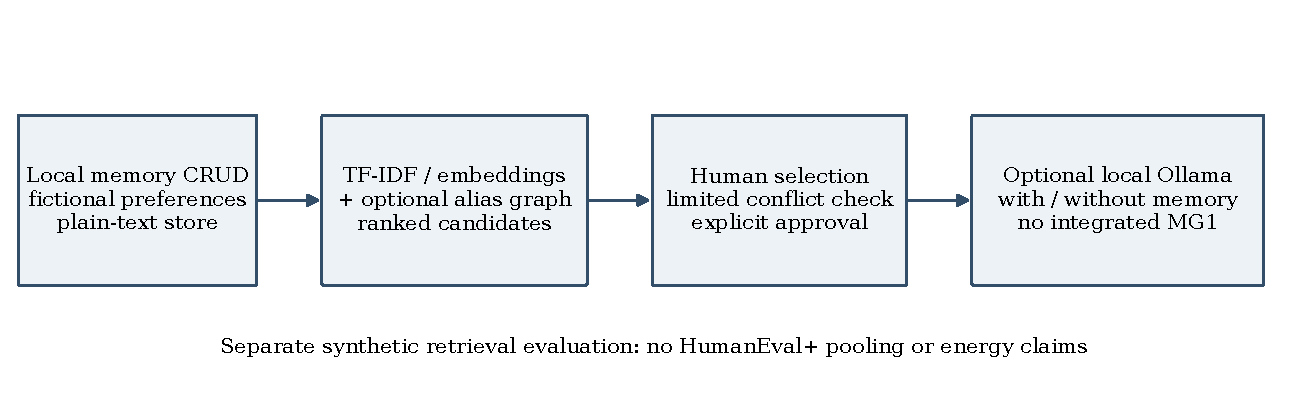
\includegraphics[width=\linewidth]{memorygraph_architecture.pdf}
\caption{Existing companion prototype, not an evaluated intervention in the
main study. Candidate selection and approval precede optional inference. The
separate saved synthetic benchmark evaluates ranking only; MG1 remains unrun.}
\label{fig:mg}
\end{figure*}

My saved synthetic evaluation contains 600 labelled query--memory pairs,
24 fictional profiles and 120 queries with five candidate memories each.
Exactly one candidate is labelled relevant. Recomputed embedding MRR is
\EmbeddingMRR{}, versus \LexicalMRR{} for TF-IDF, using the saved scores and
stable tie ordering. The embedding snapshot and data hashes are retained.
The offline lexical benchmark fits its vocabulary across the saved corpus;
the interactive lexical retriever instead fits the query and candidate memories.
MRR summarizes how early the relevant memory appears in a ranked list; it does
not score the subsequent answer. Because the two lexical pipelines fit different
vocabularies, the benchmark also does not directly measure interface ranking.
These are template-based synthetic rankings, not held-out code-generation
outcomes or estimates of real-user behavior. Grouped classifier evaluation
splits by fictional profile, but repeated templates can still supply shortcuts;
the random forest's recorded perfect synthetic result should not be read as
general memory-understanding ability.

A recorded two-prompt local demonstration supplies a pytest preference, yet
the memory-enabled response begins with \texttt{import unittest}. Both
successful API responses reach the 128-token output budget, and correctness
and energy were not scored. A preceding failed demonstration run is retained separately. This is a concrete example of availability without the intended
surface behavior, not an estimate of the prototype's benefit or its failure rate.
I do not pool the HumanEval+ study with this synthetic benchmark. An
integrated MG1 comparison remains Version 2 work.

\section{Discussion}
The experiments trace a progression from prompt design to context selection.
Prompt-Energy asked what an instruction costs to execute. Here the question is
also which instruction the model follows when several are available. The
cross-specification test makes this distinction visible: some wrong answers
satisfy a competing requirement rather than simply failing every tested
contract. Cross-scoring isolation responses provides a reference for how often
that behavior occurs without competing context. The 1.5B complete cases show an
association, while conservative treatment of incomplete generations weakens it.
Recency, repetition, pattern completion and ordinary boundary errors remain
possible explanations rather than mechanisms identified by these measurements.

Context length alone is consequently an incomplete description of the problem.
Extra relevant material may help, while competing material can introduce a
different answer that still looks reasonable. The task-bundle results suggest
that content can matter even beside matched filler, although shared tasks limit
the inference. The uncertain interruption and replay comparisons also caution
against expecting one consistent effect from a longer history or a reminder.

The retention results connect this behavioral question to efficiency. Shorter
oracle contexts have lower observed estimated energy per correct solution, but
accuracy preservation has not been established. Shorter inputs change prefill
work; wording and position can change generated output; output length and failed
attempts change the cost ratio. The oracle also avoids the work of discovering
what is relevant. A practical policy must be evaluated with that selection cost
included, rather than inherit the oracle's advantage by assumption.

Retrieval is therefore an intermediate measurement. A system must select useful
material, handle conflicts and produce an answer that applies the current
requirement. In the worked example, the target is available but the code follows
the competing boundary. In MemoryGraph's capped demonstration, the pytest
preference is available but the response uses unittest. Neither illustration
estimates a general failure rate; both explain why a good retrieval rank alone
cannot demonstrate successful utilization.

MemoryGraph offers a concrete next setting for investigating these questions.
A future comparison could measure retrieval relevance, target correctness,
preference adherence and complete computational overhead under matched
instructions and output budgets. It should also validate the adherence metric
before collecting outcomes: the all-zero registered preference score here shows
how an unsuitable formatting rule can obscure the intended question. The
existing prototype and synthetic ranking benchmark establish a starting point,
not a completed evaluation of selective memory in use.

\section{Limitations}
These results concern two small quantized models, one code benchmark and one CPU
laptop. Training-set exposure is unknown; benchmark familiarity is neither ruled
out nor inferred from a pass. Fixed task rosters, noisy eligibility selection,
one structural generation per cell and only three isolated stochastic samples
limit generalization. Shared functions connect M1 bundles and prevent robust
component-level intervals. The smaller-model effects need not predict larger
models, other quantizations, GPUs or cloud deployments.

The study developed through revisions and is partly exploratory. Registrations and dated amendments
are preserved, but the final synthesis and cross-specification audit are
posthoc. Local Git hashes support provenance, not independent public
timestamping. Family correction does not erase prior exploration. The separate
synthetic prototype benchmark is small and templated, with no user study.

Scoring depends on finite test suites, extraction and a Windows restricted
subprocess adapter. These controls are documented rather than described as a
complete adversarial sandbox. Alternative construction and similarity labels
are AI-assisted and authored; representative witnesses are not exhaustive
semantic validation. Adverse censoring weakens the principal cross-pass result.
No recognition, internal state or intentional giving-up measurement exists.

CPU-package estimates are not calibrated process-specific energy. Unrelated
work, shared baselines, clock/sampling gaps, thermal effects and approximate
post-load boundaries remain potential errors. Bootstrap intervals reflect task
variation, not measurement calibration or independent block errors. Short
requests are particularly difficult at 500 ms resolution. The incomplete
registered cache experiment prevents a completed primary energy claim.

\section{Conclusion}
I investigated how additional and competing context relates to code correctness
and inference cost in two small local language models. Testing a failed answer
against a competing specification provides information that a single pass/fail
score misses. The 1.5B complete cases show more competing-requirement failures
under competing context, although conservative assumptions about incomplete
outputs weaken that finding. Oracle retention has lower observed estimated
energy per correct solution, with accuracy preservation unresolved and several
policy differences confounded. The preference experiment adds a measurement
lesson: a rule that rejects every response cannot answer the intended retention
question. Together, these findings motivate evaluating context selection through
both the behavior it produces and its total computational cost. MemoryGraph
provides an implemented direction for that subsequent investigation.

\section{Data and Code Availability}
\begingroup\raggedright
My code is available in the
\href{https://github.com/buildgit17626-ctrl/Memory-Under-Interference-}{GitHub repository}.
This local Version 1.1 editorial revision retains the reserved Zenodo DOI
\href{https://doi.org/10.5281/zenodo.24500468}{10.5281/zenodo.24500468}
and the proposed
\href{https://github.com/buildgit17626-ctrl/Memory-Under-Interference-/releases/tag/v1.1.0}{planned v1.1.0 GitHub release}.
The DOI is reserved; its registration and public accessibility have not been
confirmed. This editorial revision preserves the scientific findings and has
not been published externally.
I will complete Zenodo publication separately. The artifacts supply code,
frozen designs, transformed raw journals,
per-task scores, numerical power/time samples, analysis tables and source/hash
mappings. Original raw evidence remains unchanged locally. Unnecessary local
paths and process/account metadata are removed only in public derivatives;
original/public hashes distinguish them. Full multi-sensor CSV mirrors are not
redistributed; the numerical CPU-package/time exports reproduce the included
energy integrations. They do not calibrate the sensor or reconstruct other
hardware channels. The archive is an analysis release, not a claim that its
sanitized files can resume the original frozen supervisor.
\par\endgroup

\section{AI-Assistance Disclosure}
I used AI assistance for setup, autonomous Ollama execution,
harness and analysis coding, distractor construction, auditing, literature
organization and manuscript drafting. I subjected AI-generated constructions
to the recorded reference/witness checks; AI assistance is not independent
scientific validation. Original report/data are licensed under CC BY 4.0 and original code
under MIT, with third-party notices retained.
\label{maintext:end}

\begingroup
\footnotesize
\setlength{\bibsep}{3pt}
\bibliographystyle{plainnat}
\bibliography{references}
\endgroup
\onecolumn
\appendix
\section{Registered Primary Contrasts and Request Inventory}
\begin{center}\small\begin{tabular}{lrrrr}
\toprule Study & Calls & API failures & Caps & Energy readings \\
\midrule
E0 & 1968 & 2 & 6 & 1966 \\
E5 & 400 & 0 & 8 & 400 \\
M1 & 1040 & 0 & 11 & 1040 \\
M2 & 400 & 0 & 1 & 400 \\
M3R2 & 1040 & 1 & 10 & 1038 \\
M3\_initial & 280 & 0 & 1 & 280 \\
R1 & 400 & 0 & 5 & 400 \\
\bottomrule
\end{tabular}
\end{center}
These are scheduled experimental requests, not retry counts. Caps are bounded-outcome
nonpasses; API failures remain separately missing for valid-input accuracy.
Energy readings are approximate post-load CPU-package observations. The revised
interference study has one missing energy window in addition to its API failure.
Pilot and partial-diagnostic counts remain separate in the archive.

The study identifiers connect these results to the frozen protocols.
E0 is the isolated strategy comparison; initial M3 is selected-task context
load; M1 is task bundling; revised M3/R2 is semantic interference; M2 is static
return-to-task interference; R1 is retention; E5 is preference placement.
The table reproduces specified primary contrasts; it does not relabel the
posthoc synthesis as a confirmatory study. Full intervals, transition IDs and
sensitivity populations are in the machine-readable archive.
E5 rows use its original strict-adherence endpoint and four-test Holm family,
not the secondary fence-tolerant metric. All-zero paired differences yield
degenerate empirical bootstrap intervals; these are not proof of population
equivalence. M1's diagnostic/exploratory comparisons and E5 secondary
correctness contrasts are supplied in the archive rather than relabelled primary.
\small\begin{longtable}{p{.075\linewidth}p{.065\linewidth}p{.26\linewidth}rrp{.18\linewidth}r}
\toprule Study & Model & Contrast & $n$ & Diff. pp & 95\% CI pp & Holm $p$ \\
\midrule
E0 & 0.5B & P3\_1 minus P1 & 163 & -2.25 & $[-7.77, 2.86]$ & 0.44696 \\
E0 & 1.5B & P3\_1 minus P1 & 164 & 2.64 & $[-1.22, 6.30]$ & 0.44156 \\
Initial M3 & 0.5B & near-minus-irrelevant averaged length & 20 & -27.50 & $[-45.00, -10.00]$ & 0.033691 \\
Initial M3 & 1.5B & near-minus-irrelevant averaged length & 20 & -2.50 & $[-17.50, 12.50]$ & 1 \\
R1 & 0.5B & lossless\_compaction minus full\_history & 40 & 5.00 & $[-7.50, 17.50]$ & 1 \\
R1 & 1.5B & lossless\_compaction minus full\_history & 40 & 0.00 & $[-15.00, 15.00]$ & 1 \\
R1 & 0.5B & oracle\_selective minus full\_history & 40 & 7.50 & $[-5.00, 22.50]$ & 1 \\
R1 & 1.5B & oracle\_selective minus full\_history & 40 & 2.50 & $[-10.00, 15.00]$ & 1 \\
R1 & 0.5B & verbatim\_replay minus full\_history & 40 & 2.50 & $[-7.50, 12.50]$ & 1 \\
R1 & 1.5B & verbatim\_replay minus full\_history & 40 & 2.50 & $[-5.00, 10.00]$ & 1 \\
M3R2 & 0.5B & near-minus-irrelevant averaged cells & 40 & -11.25 & $[-20.62, -2.50]$ & 0.056396 \\
M3R2 & 1.5B & near-minus-irrelevant averaged cells & 40 & -2.50 & $[-10.00, 4.39]$ & 0.63525 \\
M2 & 0.5B & similar minus neutral & 40 & -12.50 & $[-25.06, 0.06]$ & 0.89844 \\
M2 & 1.5B & similar minus neutral & 40 & -2.50 & $[-12.50, 7.50]$ & 1 \\
M2 & 0.5B & other\_one minus neutral & 40 & -7.50 & $[-17.50, 0.00]$ & 1 \\
M2 & 1.5B & other\_one minus neutral & 40 & 2.50 & $[-10.00, 15.00]$ & 1 \\
M2 & 0.5B & other\_three minus neutral & 40 & -5.00 & $[-17.50, 7.50]$ & 1 \\
M2 & 1.5B & other\_three minus neutral & 40 & -15.00 & $[-27.50, -2.50]$ & 0.42188 \\
E5 & 0.5B & buried minus immediate (strict adherence) & 40 & 0.00 & $[0.00, 0.00]$ & 1 \\
E5 & 1.5B & buried minus immediate (strict adherence) & 40 & 0.00 & $[0.00, 0.00]$ & 1 \\
E5 & 0.5B & replayed minus buried (strict adherence) & 40 & 0.00 & $[0.00, 0.00]$ & 1 \\
E5 & 1.5B & replayed minus buried (strict adherence) & 40 & 0.00 & $[0.00, 0.00]$ & 1 \\
\bottomrule
\end{longtable}
\normalsize

My broad starting claims about load, replay and a possible recognition--generation
gap motivated this project, but I do not test all of them in this release. Load contrasts
do not establish internal capacity; the revised retention design does not test
the original replay-rate phase diagram; and the unrun recognition/hint studies
cannot establish a know--do gap. Frozen hypotheses and amendments remain intact.

\section{Scoring, Censoring and Oracle Audit}
I re-extract saved outputs using the frozen extractor and check native
request/response measurements. Separate sandbox records cross-score 1,029
uncensored revised-interference outputs on their alternative suites, including
isolation and controls. Sixty capped per-function candidates and one merged
complete-fence candidate are scored separately; none changes the audited target
correctness outcome. This does not prove the extractor is optimal or justify
removing caps from the registered endpoint.

I retain HumanEval/32's original oracle anomaly and report an exclusion
sensitivity. Caps-as-missing and optimistic cap-pass scenarios preserve their
different denominators. Held-out eligibility sensitivity excludes the selecting
P1 sample0 from isolated-strategy comparison outcomes. The original all-task
primary estimates remain intact. Failure reasons and infrastructure-policy
outcomes are not silently converted into evidence about model knowledge.

The cross-pass complete-case comparison requires all four competing and
irrelevant cells per task. Adverse/favorable assignments bound unknown
indicators; their intervals describe assigned scenarios. The principal 1.5B
point estimate and significance are sensitive to that assignment. No claim of
missing-at-random censoring is made. Zero both-pass cells remain explicit.

\section{Energy Robustness and the Partial Cache Diagnostic}
I retain the original block baselines, drift flags and time/power windows in my
export. Start, end and midpoint subtraction are reported separately. Excluding
drift or short windows changes the retained task population; paired cost-ratio
sensitivities require covered observations in both arms. Undefined ratio draws
are reported rather than silently discarded. Total-request and approximate
post-load estimates answer different measurement questions.

E4's original feasibility pilot stops at 10 of 20 planned requests because one
response ends short of its intended workload. A separately registered JSON-array
amendment completes a 20-call pilot, then saves 76 of 400 full requests. These
workloads and pilots are not pooled. The full run has 35 cold and 41 warm
requests. Native cached-token counters show zero for the cold requests and
positive counts for the warm requests; model residency, preparation and priming
are logged separately. Matching by model, prefix and repeat yields only six
pairs in total, spread sparsely across cells. Most cells have zero or one pair;
they do not support the planned cache-energy inference. Setup/priming energy
is outside measured requests. A setup-only paused intent is not a completed
measured generation. No full E3 or U-family outcome is substituted.

\section{Companion Implementation and Reproduction Boundaries}
My pinned MemoryGraph source snapshot includes local CRUD, ranking, a fixed
alias graph, two narrow conflict categories and approval-gated optional Ollama
comparison. The archived synthetic dataset, per-pair scores and per-query
rankings permit MRR recalculation without embedding inference. Classifier
pipelines use grouped fictional-profile validation; template shortcuts remain.
No model weights, private memories, real-user records or executable trained
classifier pickles are needed in the release.

The portable reproduction script verifies release hashes, logical-call counts,
key fields and the principal paired comparisons from public records. An optional
full audit rebuild uses the supplied analysis code and dependencies. Offline
verification does not launch Ollama or regenerate embeddings. Original frozen
commit identifiers and transformation mappings remain provenance references;
sanitized archive bytes have their own checksums.

\twocolumn
\section[Representative Rendered Prompts]{\raggedright Representative Rendered Prompts}\label{app:prompts}
I selected these saved requests for HumanEval/0 on 0.5B; they are not new
prompt variants. The system message is \texttt{You are a helpful coding assistant.}
The public \texttt{examples/} directory supplies the exact UTF-8 prompt strings,
full call keys, native token counts, decoding options and SHA256 values; those
strings also occur in the archived call journals. The R1 examples below are
complete. The longer R2 and E5 layouts explicitly mark editorial omissions;
their complete unabridged strings remain in the supplement.

\subsection{Oracle-retained target, preference and query (complete)}
\lstinputlisting[basicstyle=\ttfamily\scriptsize]{../examples/r1-oracle.txt}

\subsection{Target and query without the preference (complete)}
\lstinputlisting[basicstyle=\ttfamily\scriptsize]{../examples/r1-target-query.txt}
The difference is an actual instruction difference in the collected policies,
not a length-only intervention. It helps explain why an oracle/no-history
comparison cannot isolate relevance selection.

\newpage
\subsection{Competing-context request used in the worked example (abridged)}
\lstinputlisting[basicstyle=\ttfamily\scriptsize]{../examples/r2-layout-excerpt.txt}
Only repeated copies are elided here; the exact archived request contains all
of them. They are task descriptions without implementation bodies or hidden
tests. Repetition to fill the budget, task position and explicit distractor
labelling are part of the construction and constrain its interpretation.

\subsection{Immediate preference in the placement study (abridged)}
\lstinputlisting[basicstyle=\ttfamily\scriptsize]{../examples/e5-layout-excerpt.txt}
The omitted region contains the fixed earlier-task descriptions. The wording
asks for code without explanation and does not explicitly ban Markdown fences;
the registered strict score nevertheless rejects fenced responses.

\end{document}
